\chapter{Neural Net Implementation} \label{chap:kitt_nn}
Plenty of neural network implementations are available nowadays. Nevertheless, one of the objectives of this thesis is to implement own framework capable of using the idea behind artificial feedforward neural networks. Besides prooving a knowledge of mathematical and algorithmical backgrounds, an integration of own utilities and functions is the main reason for the from-scratch implementation.

To accomplish the study objectives, the new framework must meet following requirements, which might be unusal for some of the provided implementations (mentioned in \cref{chapter:01:state_of_the_art}).

\begin{itemize}
\item ability to remove any synapse in a network and then to retrain the network of a new structure
\item ability to evaluate a network after each learning epoch and basically to provide an open-sourced learning algorithm
\item ability to illustrate a network structure and to visualize the learning process in real time (an extra property)
\end{itemize}

In this thesis, the implemented neural network framework is called \textbf{kitt\_nn} and has been developed in programming language Python. The following diagram (\ref{img:kitt_nn_package}) shows the structure of the \textit{kitt\_nn .py package}.

\begin{figure}[H]
  \centering
  \includegraphics[width=0.75\textwidth]{kitt_nn_package.png}
  \caption{kitt\_nn package : Implemented neural network framework}
  \label{img:kitt_nn_package}
\end{figure}

Moreover, the framework must have some standard functions implemented, meaning it must be capable of:

\begin{itemize}
\item initializing a feedforward network of any structure supplied by some randomly set parameters
\item fitting a model to a network (function \textit{fit()}), training a network on some data of a conventional structure
\item predicting a target of never-seen samples (function \textit{predict()}), evaluating a classification performance
\end{itemize}

The \textit{kitt\_nn} implementation is based on some general knowledge gained at school and/or from [], the idea is pretty straight forward.

\section{Structural Elements} \label{sec:structural_elements}
The overall idea is based on the object-oriented programming. There are three fundamental files containing the main classes corresponding to structural elements - a network, a neuron and a synapse (a connection). A detailed API is attached as \cref{app:code_documentation}.

\subsection*{kitt\_neuron.py} \label{ssec:kitt_neuron}
The very basic units of a neural net are called neurons. In case of artificial systems, these units are responsible for transfering all their inputs into one output. The behavior is moreless the same for all of the units, therefore a class called \textit{Neuron} implements some basic common functions.

\begin{figure}[H]
  \centering
  \includegraphics[width=0.6\textwidth]{kitt_neuron.png}
  \caption{kitt\_neuron.py : Neuron class inheritance}
  \label{img:kitt_neuron}
\end{figure}

Then, as \cref{img:kitt_neuron} shows, three classes are inherited from the \textit{Neuron} class. Some special functions, like fitting a sample in case of input layers or producing network outcome by output layers respectively, can be implemented this way, while some common functions are shared in the mother \textit{Neuron} class.

\subsection*{kitt\_synapse.py} \label{ssec:kitt_synapse}
Next, there is a class representing a neural connection - a synapse. An instance of this class takes care of the corresponding weight and remembers the two connected neurons. 

Additionally, a function called \textbf{remove\_self()} is implemented, which sets the weight to zero and removes the synapse from a database of the corresponding neural net. Then it also checks the two connected neurons, if they have some other connections remaining. If not, they are labeled as \textit{dead}, as they are not a part of the network anymore.

\subsection*{kitt\_net.py} \label{ssec:kitt_net}
The network is initialized by creating an instance of \textit{NeuralNetwork()} class from \textit{kitt\_net.py}. The initialization process is illustrated in \cref{img:kitt_net}. Basically, the only parameter is the network structure, which is expected as a \textit{.py iterable} type. 

For instance, a network with 2 input, 5 hidden and 3 output units would be created as \textit{NeuralNetwork(structure=[2, 5, 3])}. Number of hidden layers is not limited.

\begin{figure}[H]
  \centering
  \includegraphics[width=0.7\textwidth]{kitt_net.png}
  \caption{kitt\_net.py : Neural Network Initialization}
  \label{img:kitt_net}
\end{figure}

A learning algorithm is added to the initialized network thereafter (see \cref{sec:learning_algorithm}). The network class implements basic functions like \textit{fit()}, \textit{predict()} in order to be used as a classifier. Moreover, it has some additional utilities like \textit{copy\_self()} or \textit{print\_self()}, which are essential for this work (\cref{sec:gui}, \cref{sec:network_pruning_algorithm}).

\newpage
\section{Learning Algorithm} \label{sec:learning_algorithm}
In general, learning algorithms represent the part of artificial systems that makes them behave intelligently when accomplishing a specific task. In classification, the goal of learning is to fit some training data to a model, which generally means to set some parameters based on the chosen classification approach.

In case of feedforward neural networks, the learning goal is to find optimal values for two groups of parameters - \textit{weights} and \textit{biases} (described in \cref{sec:intro_to_nn}).

A popular algorithm called \textit{Backpropagation} has been chosen to deal with the learning task. The backpropagation abbreviation stands for \textit{backward propagation of errors}. The approach is based on an optimization method called \textit{Gradient Descent Algorithm (GDA)}. Method details can be found in \citep{online:nn_demystified}.

In this work, the implementation is made to be compatible with the \textit{kitt\_nn} network (\cref{sec:structural_elements}) and adjusted to the needs of the developed pruning algorithm (\cref{sec:network_pruning_algorithm}). The learning process is summarized by the following flowchart \ref{img:backpropagation} and the procedure follows algorithmical steps in \citep{online:nn_demystified}.

\begin{figure}[H]
  \centering
  \includegraphics[width=1\textwidth]{backpropagation.png}
  \caption{Training process flowchart}
  \label{img:backpropagation}
\end{figure}

\begin{description}
\item[$ T_1 $] : Threshold for a terminating condition based on a learning error. If the error is reduced to be lower than this threshold, the learning process is stopped.
\item[$ T_2 $] : Threshold for a terminating condition based on number of iterations (epochs). The learning process is stopped after a specified number of epochs, no matter how successful the training has been.
\end{description}

\subsection{Using Mini-batches} \label{ssec:minibatches}
The idea of multilayer perceptrons (\cref{sec:intro_to_nn}) is described on propagating one sample through a network. However, using the matrix arithmetic, more samples can be send to the network, while activities and activations of neurons in one layer are computed at the same time for all of those samples.

This group of samples is called \textit{a mini-batch}. Using mini-batches can speed up the process, however it can bring some problems with finding the right solution by the \textit{Gradient Descent} method (evident from \cref{eq:batch_gd}). Usually, the mini-batch size is left as a training parameter. In this work, it is set to \textit{10}.

\subsection{Matrix Notation} \label{ssec:matrix_notation}
Assuming feedforward neural networks (multilayer perceptrons), the following notation is used in this study.

\begin{description}
\item[$ X $] : network input: $ m $-by-$ n $ matrix, where $ m $ is the number of samples and $ n $ is the size of one sample
\item[$ W^{(i)} $] : $ p $-by-$ r $ matrix of weights for synapses from neurons in layer $ i $ (layer of $ p $ neurons) to neurons in layer $ (i+1) $ (layer of $ r $ neurons)
\item[$ Z^{(i+1)} $] : $ r $-by-$ m $ matrix of activities for neurons in layer $ (i+1) $ (layer of $ r $ neurons), $ m $ is the number of processed samples at the same time (see \cref{ssec:minibatches})
\item[$ f() $] : activation function
\item[$ f'() $] : activation function derivative
\item[$ \hat{y} $] : network predicted output: $ q $-by-$ m $ matrix, where $ q $ is the number of output neurons and $ m $ is the number of processed samples ($ \hat{y} = f(Z^{(j)}) $, where $ j $ is the number of layers)
\item[$ y $] : network actual output (known targets): $ q $-by-$ m $ matrix, where $ q $ is the number of output neurons and $ m $ is the number of processed samples
\item[$ \delta^{(i)} $] : error vector of length $ p $ for $ p $ neurons of $ i^{th} $ layer
\end{description}

\subsection{Forward Propagation} \label{ssec:forward_propagation}
With reference to previous sections, the following equations are used to propagate a batch of samples $ X $ through a network and get a corresponding matrix of outputs $ \hat{y} $.

\begin{align}
Z^{(2)} = X \cdot W^{(1)}
\end{align}

\begin{align}
Z^{i+1} = a^i \cdot W^i
\end{align}

\begin{align}
a^{(i)} = f(Z^{(i)})
\end{align}

\begin{align}
\hat{y} = f(Z^{(j)})
\end{align}

\subsection{Error Calculation} \label{ssec:error_calculation}
To get an idea about how wrong the networks predictions are, the network needs a teacher. For this reason the learning is called \textit{supervised}, as there is a batch of training data with known targets. Comparing the predictions with the correct targets, one can calculate a prediction error. 

The prediction error of the propagated batch of samples is expressed as a cost function $ J $. The goal is to minimize $ J $.

\begin{align} \label{eq:cost_function}
J = \displaystyle{\sum_{k=1}^m} \frac{1}{2}(y_k - \hat{y}_k)^2
\end{align}

\subsection{Parameters Update} \label{ssec:parameters_update}
Knowing the prediction error, the goal of the learning algorithm is to update the network weights and biases in order to reduce the error for next prediction.  It is known, that some combination of the parameters makes $ J $ (\cref{eq:cost_function}) minimal. There is no chance to check all possible combinations for bigger networks, therefore \textit{GDA} is used here.

Partial derivatives $ \frac{dJ}{dw} $ for all weights $ w $ of chosen weights matrix $ W^{(i)} $ belonging to layer $ i $ are computed and set equal to zero ($ \frac{dJ}{dw} = 0 $). Applying this on a mini-batch, we get $ m $ derivatives $ (\frac{dJ}{dW^{(i)}})_k $ for $ m $ input samples. 

\textit{GDA} is then applied on the summation of these derivatives and so all examples are considered as one (\cref{eq:batch_gd}). In human language, one can understand it as every sample has a vote on how to find the minimal error and the result is obtained as a compromise.

\begin{align} \label{eq:batch_gd}
\frac{dJ}{dW^{(i)}} =  \displaystyle{\sum_{k=1}^m} (\frac{dJ}{dw})_k
\end{align}

There are three main issues (\cref{img:gda_problems}) preventing this approach from being perfect. However, as the brute force algorithm is uncomputable, this method is chosen.

\begin{figure}[H]
  \centering
  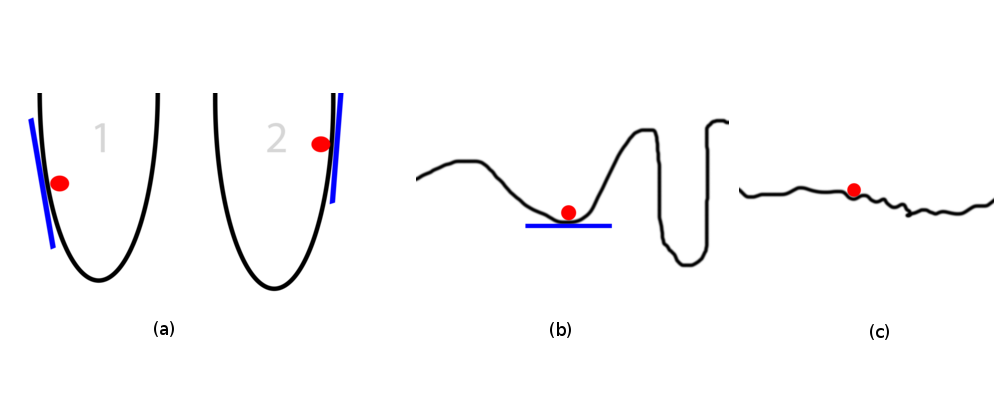
\includegraphics[width=0.85\textwidth]{gda_problems.png}
  \caption{GDA issues \citep{online:nn_demystified} (a) slopes are too big, (b) local minimums, (c) slopes are too small}
  \label{img:gda_problems}
\end{figure}


Having several layers of a network results in several weights (and biases) mattrices, while the goal is to find optimal parameters of overall network. In order to compute optimal parameters in all of the mattrices, the sum rule in differentation (\cref{eq:sum_rule}) followed by the chain rule (\cref{eq:chain_rule}) are applied.

\begin{align} \label{eq:sum_rule}
\frac{\delta}{\delta x} (u+v) = \frac{\delta u}{\delta x} + \frac{\delta v}{\delta x}
\end{align}

\begin{align} \label{eq:chain_rule}
(f \circ g)' = (f' \circ g) \cdot g'
\end{align}

Due to these properties, the error obtained at the network output (\cref{ssec:error_calculation}) is propagated backwards layer by layer through the network (\cref{eq:error_backprop}) and derivatives $ \frac{dJ}{dW^{(i)}} $ for all $ i $ layers are found (\cref{eq:part_derivative}).

\begin{align} \label{eq:error_backprop}
\delta^{(i)} = \delta^{(i+1)} \cdot (W^{(i)})^T \cdot f'(Z^{(i)})
\end{align}

\begin{align} \label{eq:part_derivative}
\frac{dJ}{dW^{(i)}} = (a^{(2)})^T \cdot \delta^{(i+1)}
\end{align}

Due to issues shown on \cref{img:gda_problems}, there are no garranties of getting a good solution, getting a solution in a finite number of iterations and even not of getting a solution at all. However, this approach is considered as the state of the art nowadays.

In this work, it is implemented in \textit{Python}, using mostly the \textit{numpy} library for the expensive matrix operations. The implementation complies with the needs of the pruning algorithm from \cref{sec:network_pruning_algorithm} and is fully compatible with the \textit{kitt\_nn} framework for any type of data.

\section{Graphical User Interface} \label{sec:gui}
The graphical interface has been implemented as an extension for \textit{kitt\_nn} framework. It is actually not strictly needed for this study, but it provides some interesting functions worth of being introduced. Anyway, any type of visualization usually helps to understand a problem better.

\begin{figure}[H]
  \centering
  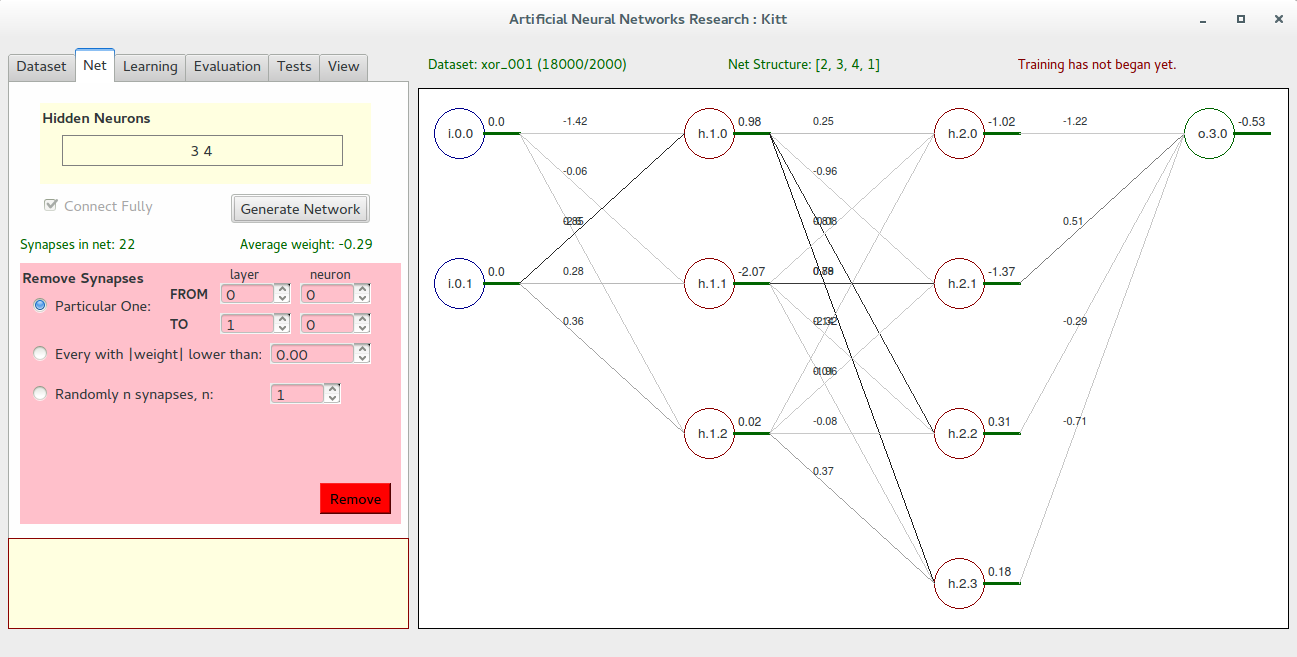
\includegraphics[width=1.0\textwidth]{gui_screen.png}
  \caption{Screenshot of the graphical user interface}
  \label{img:gui_screen}
\end{figure}

This GUI is capable of:
\begin{enumerate}
\item Loading a dataset in a specific form and, if possible, visualizing it (see XOR data in \cref{img:data_xor} for an example, this image is generated by the GUI).
\item Generating a network of any hidden structure. The input and output layers are defined by the chosen dataset. The network is then visualized (as shown in \cref{img:gui_screen}).
\item Removing synapses of the network, while the visualization is interactive with the structure changes.
\item Training the network, while the visualization is interactive, so the weights changes can be seen online.
\item Performing some tests and plotting basic evaluations.
\item Adjusting the visualization view in sense of zooming, resizing or changing colors.
\end{enumerate}

The visualization is not that useful for huge network structures, however, it can be essential at some points of the workflow. Nevertheless, it is considered as the very fist version for now and aimed to be upgraded in the future.

\newpage
\section{Network Pruning Algorithm} \label{sec:network_pruning_algorithm}

\subsection{Idea}

\subsection{Realization}

\begin{figure}[H]
  \centering
  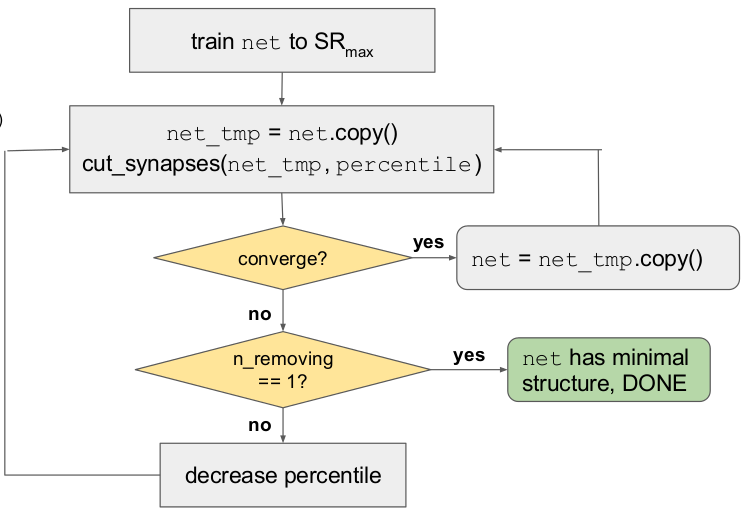
\includegraphics[width=1.0\textwidth]{pruning_algorithm.png}
  \caption{The Pruning Algorithm}
  \label{img:pruning_algorithm}
\end{figure}

\subsection{Testing Datasets}

\subsubsection*{XOR Dataset}

\begin{figure}[H]
  \centering
  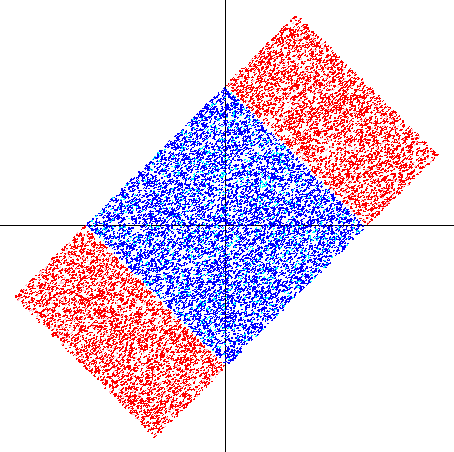
\includegraphics[width=0.7\textwidth]{data_xor.png}
  \caption{2D XOR Data illustration}
  \label{img:data_xor}
\end{figure}

\begin{figure}[H]
  \centering
  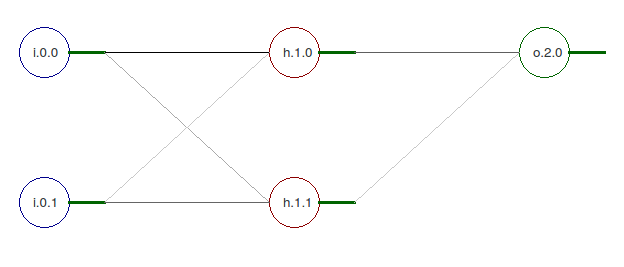
\includegraphics[width=0.6\textwidth]{xor_min_structure_1.png}
  \caption{XOR min structure 1}
  \label{img:xor_min_structure_1}
\end{figure}

\begin{figure}[H]
  \centering
  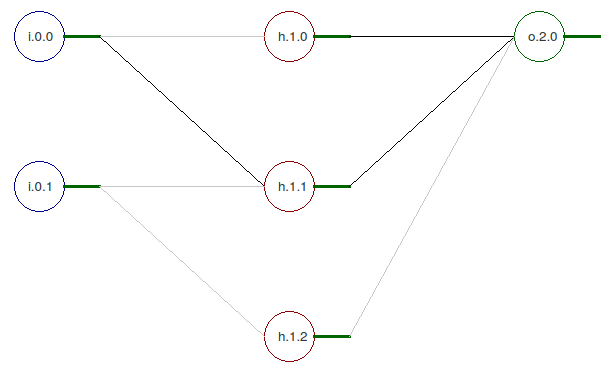
\includegraphics[width=0.6\textwidth]{xor_min_structure_2.png}
  \caption{XOR min structure 2}
  \label{img:xor_min_structure_2}
\end{figure}

\subsubsection*{MNIST Dataset}

\begin{figure}[H]
  \centering
  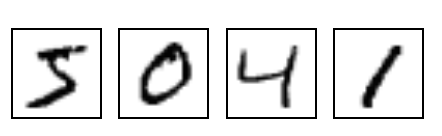
\includegraphics[width=0.7\textwidth]{data_mnist.png}
  \caption{MNIST Data illustration}
  \label{img:data_mnist}
\end{figure}

\subsection{Minimal Structures Utilization}
further MNIST analysis

figures, tables

4-5 pages